\documentclass[a4paper,12pt]{article}

\usepackage[utf8]{inputenc}
\usepackage{fullpage}
\usepackage{parskip}
\usepackage{amsmath}
\usepackage{hyperref}
\usepackage{graphicx}
\usepackage[croatian]{babel}
\usepackage[T1]{fontenc}

% TODO: align, verbatim, equation blocks

\renewcommand{\figurename}{Slika}
\newcommand{\engl}[1]{(engl.~\emph{#1})}

\title{Rangirajući pretraživač dokumenata - Infinity}
\author{Marko Budiselić}
\date{30.11.2015.}

\begin{document}

\maketitle

\section{Pretprocesiranje}

Bitan segment analize teksa je predprocesiranje. Predprocesiranje počinje s podjelom dokumenta na riječi \engl{tokenization}. Implementiran je jednostavni tokenizator koji prvo zamijenjuje posebna znakove s prazninama, nakon toga odbacuje riječi duže od 25 znakova (25 je nastao subjektivnom procjenom) i na kraju se radi svođenje riječi na jednostavniji oblik \engl{stemming}. Korišten je Snowball (Porter2) stemmer zato što je manje agresivan od Lancaster stemmer-a, a brži od Porter stemmer-a. Uvođenjem stemmer-a naraslo je vrijeme izvođenja pretprocesiranja i to za $\sim$4 puta (koristi se stemming Python modul). Trebalo bi koristiti neku brzu C/C++ implementaciju stemming postupka. Nije se koristio lematizator zato što je bitno očuvati riječi što je moguče više onakve kakve jesu. Primjerice, ne bi bilo dobro zamijeniti \textit{is} s \textit{be}, jer je korisnik možda baš htio dokumente gdje se pojavljuje \textit{is}. Lematizator bi \textit{is} riječ zamijenio s riječi \textit{be} i tu bi se izbugila informacija (opet subjektivna procjena). Kada bi postojala potreba za lematizatorom tada bi se uz Python koristio spacy lematizator i to zato što je brži u odnosu na, primjerice, nltk lematizatora. 

\section{Algoritmi}

\subsection{Bag of words}

Dvije su osnovne strukture podatatak unutar algoritma. \textit{Bag of words} unutar svakog dokumenta broji koliko se puta pojedina riječ pojavila unutar tog dokumenta. \textit{Bag of documents} za svaku riječ broji koliko se puta pojavila u pojedinom dokumentu. Stvari su slične, ali omogučuju da se algoritam izvede u složenosti \textit{(broj riječi upita} * \textit{broj dokumenata u kojima se pojavljuje riječ)}. Pristigli upit najprije se pretprocesira, potom se za svaku riječ i za svaki dokument unutar kojeg se ta riječ pojavljuje računa normalizirana težina. Za svaku riječ  gleda se koliko puta se ona pojavljuje unutar dokumenta i onda se ta vrijednost normalizira s veličinom dokumenta. Na taj način se postiže da kraći dokumenti u kojima broj pojavljivanje pojedine riječi čini veći postotak unutar dokumenta imaju snažniji utjecaj nego dokumenti u kojima se rijeđe pojavljuje dotična riječ. Na kraju se sortiraju dobiveni dokumenti prema izračunatim težinama. Dobre strane algoritma su brzina, jednostavnost, normalizacija, a mana je što se ne uzima nikakva globalna informacija o zastupljenosti riječi unutar cijelog skupa dokumenata. Uvijet koji bi trebao biti zadovoljen je da ne postoji dokument unutar kojeg se nalaze sve riječi iz korpusa. U suprotnom će algoritam sporije raditi od očekivanog, ali pretpostavka je da se to neće dogoditi. Na danom skupu dokumenata, vrijeme izvođenja algoritma je rada veličine 1ms i ne bi trebalo postati drastično veće na skupu od, primjerice, reda veličine 1M dokumenata.

\subsection{Vector space}

\subsection{Binary independence}

\section{Implemntacija}

Svaki algoritam tipa je \textit{IRAlgorithm}. Taj tip posjeduje četiri metode. \textit{config} putem koje se prima nekakva konfiguracija algoritma, ako takva za dani algoritam postoji. \textit{preprocess\_all} kroz koju se radi predprocesiranje svih dostupnih dokumenata. \textit{preprocess\_one} putem koje se radi predprocesiranje samo jednog novog dokumenta. I, \textit{run} koja vrača konkretne rezultate. Kako bi se izbjeglo pokretanje predprocesiranja svaki put kada se treba pokrenuti neki algoritam uveden je razred AlgorithmBox koji posjeduje instance svih dostupnih algoritama u varijabli \textit{available\_algorithms}. U varijabli \textit{prepared\_algorithms} nalaze se samo one instance algoritama za koje je već proveden proces predprocesiranja. Varijabla \textit{prepared\_algorithms} se prilikom svakog postavljanja novih dokumenata kroz \textit{setter files} postavi na prazni riječnik. Na taj način se postiže da se kod idučeg dohvačanja nekog algoritma ponovno forsira proces predprocesiranja. Ukoliko se dodao samo jedan dokument onda se samo pozove metoda \textit{preprocess\_one} nad svim algoritmima koji su unutar riječnika \textit{prepared\_algorithms}. Mana ovog pristupa je što svaki algoritam za sebe drži kopiju svih dokumenata i ponavljanje predprocesiranja za svaki algoritam posebno. Prednost je, svojstvo da svaki algoritam ima izolirani skup podataka s kojim može činiti što je već potrebno kako bi algoritam valjano radio. Odlučio sam se za taj pristup zato što je memorija manji problem od nekakve jednostavnosti korištenja i važnosti da je svaki algoritam za sebe izoliran. Jedna od mana trenutne implementacija je i što se dokumenti pamte unutar riječnika. Optimalnije bi bilo pamtiti dokumente unutar liste, te imati potporne strukture podataka kao što su riječnici u kojima bi se pamtilo primjerice na kojoj poziciji u listi je određeni dokument.

\section{Upute za pokretanje}

\url{https://infinity.buda.link}

TODO: source setup.py

TODO: objasniti konzolu (history)

\section{Produkcijska okolina}

Svi upiti klijenata dolaze na Nginx load balancer koji ima izrazito veliku propusnost. Nakon toga load banancer prosljedjuje upit na worker instance koje svaka za sebe imaju cijeli dataset i znaju vratiti odgovarajuci rezultat. Dataset worker instance preuzimaju od db interface instance, a ne direktno iz baze. Trenutno je u deploymentu samo jedna instanca sucelja prema bazi, ali u produkciji tu moze biti opet load balancer i vise instanci interface-a prema bazi podataka. Baza podataka je MongoDB, takodjer samo jedna instanca, no u praksi tu moze doci mongo replica set ili mongo shard cluster.

Kao sto se vidi na slici \ref{production_environment}, sve instance imaju simbolicka imena (FQDN). To je takodjer izrazito bitno jer se time postize transparentnost pristupa i migracijska transparentnost. U konkretnoj implementaciji sva imena su definirana u /etc/hosts file-u na deploy stroju, no u produkciji ce imene biti definirana na redundantnim DNS serverima.

\begin{figure}[!htbp]
\begin{center}
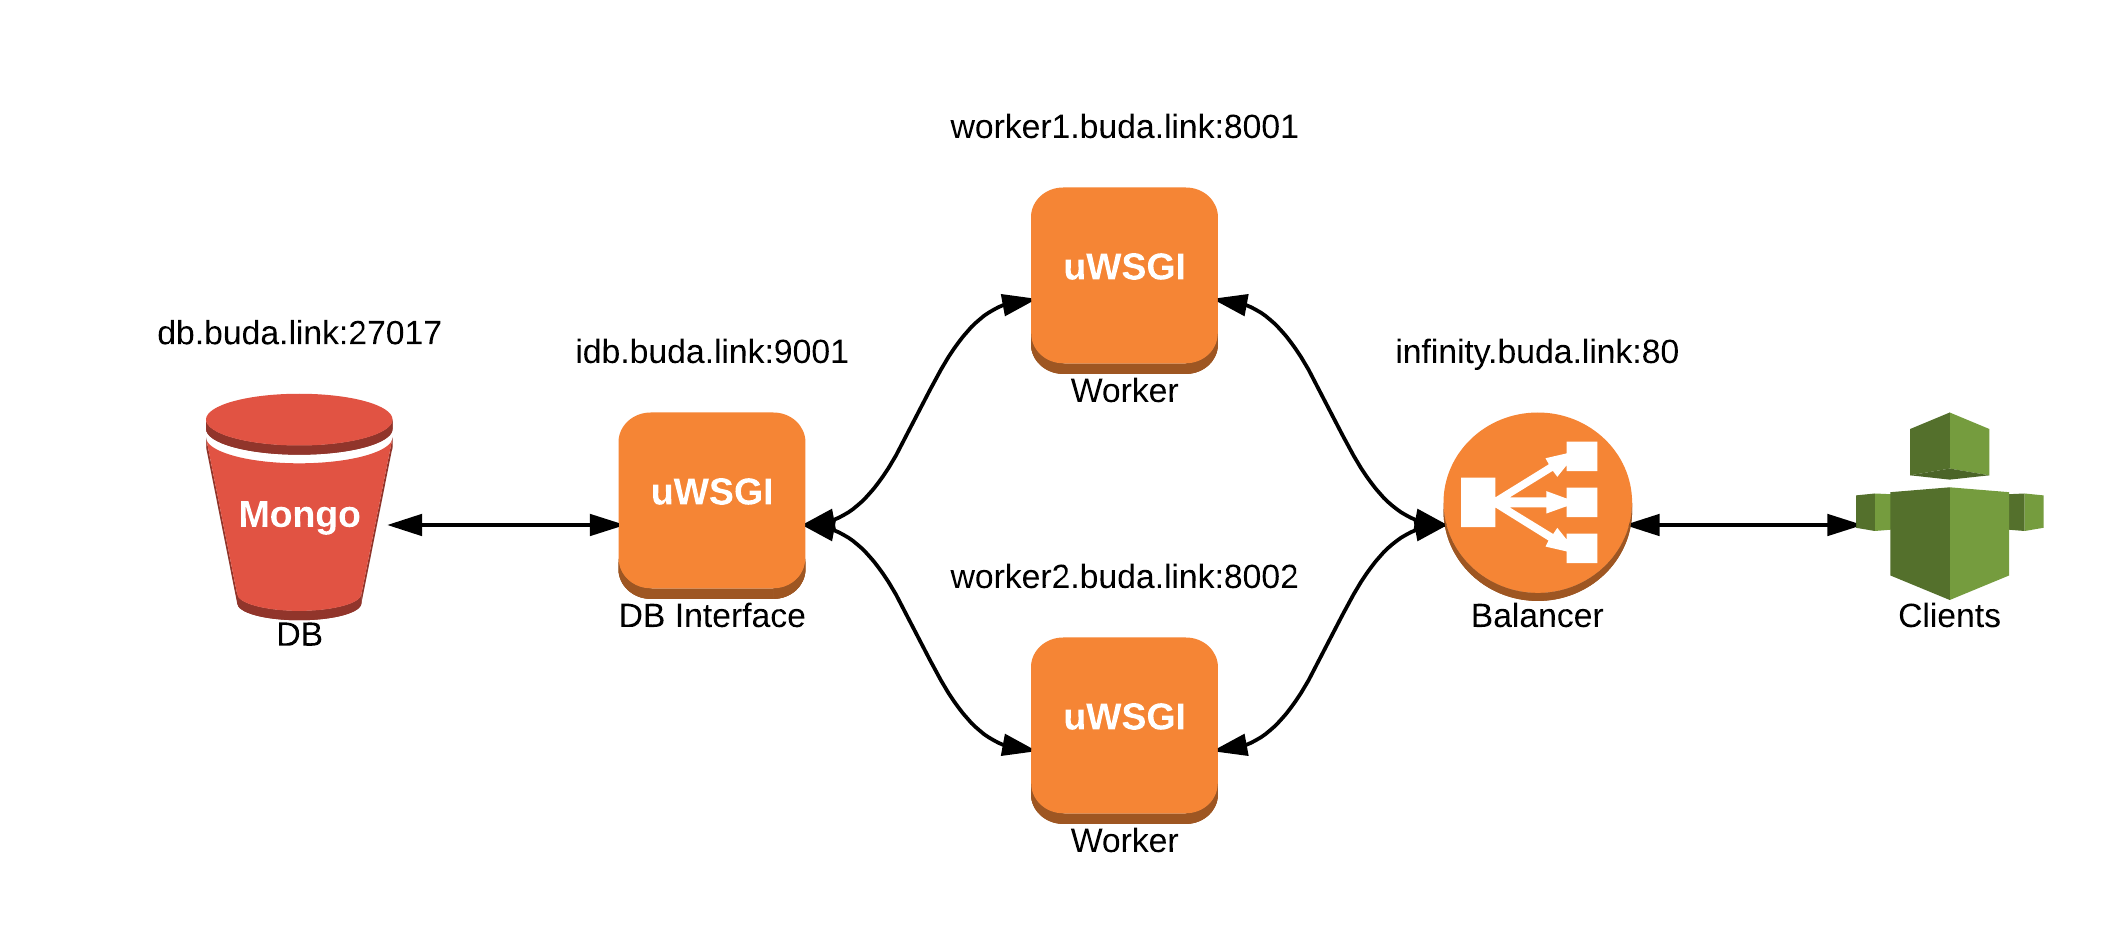
\includegraphics[width=\textwidth]{infinity.png}
\end{center}
\caption{Produkcijska okolina}\label{production_environment}
\end{figure}

\section{Web sučelje}

TODO: Angular + materializecss

TODO: nekakva slika sučelja

\vspace{1cm}
P.S.
\\[0.3cm]
infinity $>$ gugol

\bibliographystyle{plain}
\bibliography{bibliography.bib}
\end{document}